In a distributed system the interaction between clients plays an important role. Setting up scenarios with real clients becomes unfeasible due to the complexity that a distributed system brings with it. To analyse and debug the state or a problem of a client, a deterministic environment is required, where a state or a problem can be easily reproduced.
Thus, simulation tools are needed where multiple virtual instances can be spawned and monitored easily. The virtual instances have to interact with each other like like they would do in a real environment. Also, the virtual instances shall provide information, e.g. data that is sent, without modifying the actual implementation. Last but not least, the virtual instances shall live in a controllable environment where all instances can be accessed, started and stopped at the same time. 

This chapter describes the tools that have been developed to analyse and debug the implementation of Mitosis. \vref{fig:anl-overall-stack} presents the stack of the developed tools.

Each component is described briefly in the following before going further into details.

\begin{itemize}
    \itembf{Simulation} The core component that spawns virtual instances and runs Mitosis in each of it. The communication between the virtual instances is mocked, thus a physical connection is not required. The virtual instances can be orchestrated through a \textit{Scenario} that the Simulation is executing.
    \itembf{Visualisation} Visualises the output that is provided by the Simulation component. Also allows interaction with each virtual instance. Inspector tools allow to inspect the state of each instance. The virtual instances are visualised as a force directed graph.
    \itembf{CLI-Import} Parts of the results of the CLI can be imported into the Visualisation so the result can be restored as a force directed graph and further analysed.
    \itembf{Realtime Visualisation} A dedicated test application that executes Mitosis in a real environment reports its state to a server. The visualisation creates a graph based on the reported clients in almost realtime. 
    \itembf{CLI} Executes the simulation in a Node.js environment and does not have any graphical feedback. Parameterized execution of scenarios allows benchmarking. Results are exported as files as soon as the execution is done.
\end{itemize}

\begin{figure}
\centering
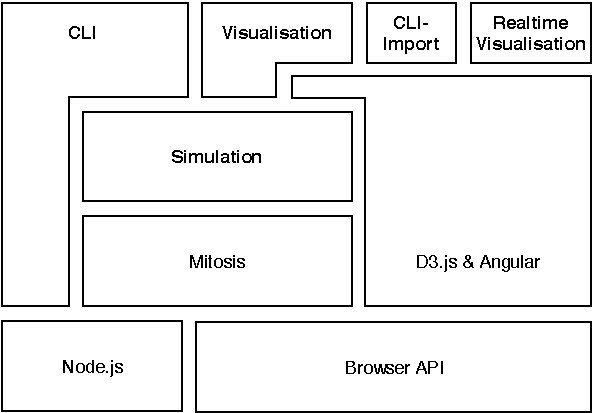
\includegraphics[width=0.7\textwidth]{graphics/analysis-tools/analysis-tools.pdf}
\caption{Stack}
\label{fig:anl-overall-stack}
\end{figure}